\documentclass[a4paper,11pt,headsepline]{report} % scrreprt würde auch gehen

\usepackage{titling}

%----------------- PDF CONFIG ----------------- %
\pdfinfo{    
     /Title     (Scientific Project) 
     /Subject   (Zigbee Praktikum)    
     /Author    (Benedikt Heuser) 
     /Keywords  (HSRM)      
} 

\title{Entwicklung eines Zigbee Praktikums unter Verwendung von OpenSource Technologie}
\author{Benedikt Heuser}
\date{25.04.2022}



%----------------- PAKETE INKLUDIEREN ----------------- %

\usepackage[enable]{easy-todo} % Bietet eine art TODO Liste an; Zum bauen des abgabebereiten Dokumentes sollte die Option enable durch disable ersetzt werden!

\usepackage{geometry} % Packet für Seitenrandabständex und Einstellung für Seitenränder
\usepackage[ngerman]{babel} % deutsche Silbentrennung
\usepackage{blindtext} % Für den Beispieltext

\usepackage{booktabs} % entzerrt die Tabellenzeilen und bietet verschieden dicke Unterteilungslinien
\usepackage{longtable} % Tabellen können sich nicht über mehrere Seiten 
\usepackage{graphicx} % kann LaTeX Grafiken einbinden
%\usepackage{parskip}
\usepackage{xstring} % Für das FakeSmallCaps

\usepackage[utf8]{inputenc}
%\usepackage[applemac]{inputenc} % Umlaute unter Mac werden automatisch gesetzt
\usepackage[T1]{fontenc} % Zeichenencoding
\usepackage{lmodern} % bessere typographische Qualität 
\frenchspacing % Schaltet den zusätzlichen Zwischenraum ab; Wird mit ngerman-babel schon geladen
\usepackage{fix-cm}
\usepackage{hyperref} % verwandelt alle Kapitelüberschriften, Verweise aufs Literaturverzeichnis und andere Querverweise in PDF-Hyperlinks
\usepackage{color}
\usepackage[table]{xcolor}
\usepackage{enumitem}
\usepackage{url}
\usepackage{acronym}
\usepackage[ddmmyyyy,hhmmss]{datetime}
\renewcommand{\dateseparator}{.}
\usepackage{tabu} % Tabellen nutzen
\usepackage{multirow}
\usepackage{booktabs}
\usepackage{setspace} % to use \singlespacing\onehalfspacing\doublespacing
\usepackage{mathtools}
\usepackage{rotating} % For sidewayfigures
\usepackage{caption} % For centering the Captions if more than one Line
\captionsetup{justification=centering,margin=3em} % Set centering for captions as default
\usepackage{charter} % modernere Serifen Font
\usepackage[nottoc]{tocbibind}
\usepackage{float}
\usepackage[many]{tcolorbox}
\usetikzlibrary{calc}

%----------------- BibLaTeX ----------------- %
\usepackage[
backend=bibtex,
style=alphabetic
]{biblatex}
\bibliography{literatur}

%----------------- LISTINGS ----------------- %
\usepackage{listings}

% LSTCOLORS
\definecolor{background}{HTML}{F1F1F1}

% Genrell Settings
\lstset{
  captionpos              = b,
  basicstyle              = \footnotesize\ttfamily,
%  backgroundcolor         = \color{background},
  numbers                 = left,
  numberstyle             = \scriptsize\color{background!70!black},
  stepnumber              = 1,
  numbersep               = 3ex,
  showstringspaces        = false,
  breaklines              = true,
  framesep                = 1ex,
  frame                   = l,%trb,
  framerule               = .35ex,
  xleftmargin             = 1.37ex,
%  frameround              = tttt,
  rulecolor               = \color{black},
  commentstyle            = \color{darkgray!80},
  escapeinside            = {<@[}{]@>}, % You can Escape inside the LST with <@[ ESCAPED_TEXT ]@>
  lineskip                = {-1.2pt},
  aboveskip               = {2em},
  belowskip               = {1em},
}

% PHP
\definecolor{dkgreen}{rgb}{0,.6,0}
\definecolor{dkblue}{rgb}{0,0,.6}
\definecolor{dkyellow}{cmyk}{0,0,.8,.3}
\definecolor{dkorange}{rgb}{1.0, 0.5, 0.0}

\lstset{
  language         = PHP,
  keywordstyle     = \color{dkblue},
  stringstyle      = \color{red},
  identifierstyle  = \color{dkgreen},
  emph             = [1]{php},
  emphstyle        = [1]\color{black},
  emph             = [2]{if,and,or,else,null,NULL},
  emphstyle        = [2]\color{dkorange},
  emph             = [3]{class,implements,namespace,public,private,protected,function,return,new,throw,try,catch,as,instanceof},
  emphstyle        = [3]\color{dkblue},
  morekeywords     = {class,implements,namespace,public,private,protected,function,return,new,throw,try,catch,as,instanceof},
}


% JSON  
\colorlet{punct}{red!60!black}
\definecolor{delim}{RGB}{20,105,176}
\colorlet{numb}{magenta!60!black}

\lstdefinelanguage{json}{
%  stringstyle      = \color{orange},
%  morestring       = [b]",
  literate         =
   *{0}{{{\color{numb}0}}}{1}
    {1}{{{\color{numb}1}}}{1}
    {2}{{{\color{numb}2}}}{1}
    {3}{{{\color{numb}3}}}{1}
    {4}{{{\color{numb}4}}}{1}
    {5}{{{\color{numb}5}}}{1}
    {6}{{{\color{numb}6}}}{1}
    {7}{{{\color{numb}7}}}{1}
    {8}{{{\color{numb}8}}}{1}
    {9}{{{\color{numb}9}}}{1}
    {:}{{{\color{punct}{:}}}}{1}
    {,}{{{\color{punct}{,}}}}{1}
    {\{}{{{\color{delim}{\{}}}}{1}
    {\}}{{{\color{delim}{\}}}}}{1}
    {[}{{{\color{delim}{[}}}}{1}
    {]}{{{\color{delim}{]}}}}{1}
    {"}{{{\color{red}{"}}}}{1}, % make " red
}

\lstdefinelanguage{yaml}{
  keywords        = {true,false,null},
  comment         = [l]{\#},
  morecomment     = [s]{/*}{*/},
  morestring      = [b]',
  morestring      = [b]",
}


%----------------- FARBEN DEFINIEREN ----------------- %
% ~Hochschulfarben~
% Primary Colors
\definecolor{hsrmRed}{rgb}{0.882352941,0,0.098039216}
\definecolor{hsrmRedDark}{rgb}{0.588235294,0,0.058823529}
\definecolor{hsrmWarmGreyDark}{rgb}{0.274509804,0.254901961,0.235294118}
\definecolor{hsrmWarmGreyLight}{rgb}{0.666666667,0.647058824,0.62745098}

% Secondary Colors
\definecolor{hsrmSec1}{rgb}{0,0.588235294,0.509803922}
\definecolor{hsrmSec1Dark}{rgb}{0,0.392156863,0.31372549}
\definecolor{hsrmSec1Comp}{rgb}{0.294117647,0.745098039,0.882352941}
\definecolor{hsrmSec1CompDark}{rgb}{0.196078431,0.490196078,0.568627451}

\definecolor{hsrmSec2}{rgb}{0.607843137,0.764705882,0.156862745}
\definecolor{hsrmSec2Dark}{rgb}{0.411764706,0.490196078,0.098039216}
\definecolor{hsrmSec2Comp}{rgb}{0.254901961,0.156862745,0.509803922}
\definecolor{hsrmSec2CompDark}{rgb}{0.176470588,0.098039216,0.333333333}

\definecolor{hsrmSec3}{rgb}{0.509803922,0.078431373,0.31372549}
\definecolor{hsrmSec3Dark}{rgb}{0.338345865,0.058823529,0.196078431}
\definecolor{hsrmSec3Comp}{rgb}{1,0.509803922,0}
\definecolor{hsrmSec3CompDark}{rgb}{0.666666667,0.333333333,0}

% Custom Colors
\definecolor{gray}{gray}{0.95} % Listingsbackground
\colorlet{darkgray-light}{darkgray!90}

% Farbskala - um zB Prioritäten darzustellen
\definecolor{colorscale-green}{HTML}{DBFF33}
\definecolor{colorscale-yellow}{HTML}{FFF033}
\definecolor{colorscale-orange}{HTML}{FFBD33}
\definecolor{colorscale-dkorange}{HTML}{FF8A33}
\definecolor{colorscale-red}{HTML}{FF5733}
\definecolor{colorscale-gray}{gray}{.75}

%----------------- NEW Commands ----------------- %
% Eigener kurzer LoremIpsumDummyText
\newcommand{\sblindtext}{Dies hier ist ein Blindtext zum Testen von Textausgaben. Wer diesen Text liest, ist selbst schuld. Der Text gibt lediglich den Grauwert der Schrift an. Ist das wirklich so? Ist es gleichg\"{u}ltig, ob ich schreibe: ``Dies ist ein Blindtext'' oder ``Huardest gefburn''? Kjift $-$ mitnichten!}

% Define conclusionbox
\newcommand{\conclusionbox}[1]{\begin{center}\colorbox{darkgray!20}{\parbox{.9\textwidth}{#1}}\end{center}}

% Chapter Summary
\newcommand{\chaptersummary}[1]{\vspace{2em}\colorbox{darkgray-light}{\hspace{.03\textwidth}%
\parbox{.94\textwidth}{\vspace{.25em}%
\setlength{\parskip}{1.2ex}\bfseries\color{white}%
#1\vspace{1em}}%
\hspace{.03\textwidth}}%
\vspace{2em}}

% Fake Small Caps
\newcommand{\fakesmallcaps}[1]{\StrLeft{#1}{1} {\scriptsize\uppercase{\StrGobbleLeft{#1}{1}}}}

% Trenner
\newcommand{\trenner}{\centerline{\textcolor{risk-gray}{\rule{0.7\textwidth}{.4pt}}}}

% Table Midrule
\newcommand{\customcmidrule}[2]{\arrayrulecolor{#2}\cmidrule(l{1.5em} r{1.5em}){#1}\arrayrulecolor{black}}

% My Quote
\newenvironment{customquote}{\begin{quote}\raisebox{-.4\height}{{\Huge\color{darkgray-light} ''}}}{\end{quote}}

\tcbset{mystyle/.style={
  breakable,
  enhanced,
  outer arc=0pt,
  arc=0pt,
  colframe=colorscale-yellow,
  colback=colorscale-yellow!20,
  attach boxed title to top left,
  boxed title style={
    colback=colorscale-yellow,
    outer arc=0pt,
    arc=0pt,
    top=3pt,
    bottom=3pt,
    },
  fonttitle=\sffamily
  }
}

\tcbset{mystyle1/.style={
  breakable,
  enhanced,
  outer arc=0pt,
  arc=0pt,
  colframe=colorscale-orange,
  colback=colorscale-orange!20,
  attach boxed title to top left,
  boxed title style={
    colback=colorscale-orange,
    outer arc=0pt,
    arc=0pt,
    top=3pt,
    bottom=3pt,
    },
  fonttitle=\sffamily
  }
}
\newtcolorbox[auto counter,number within=section]{Hinweis}[1][]{
  mystyle,
  title=Hinweis,
  overlay unbroken and first={
      \path
        let
        \p1=(title.north east),
        \p2=(frame.north east)
        in
        node[anchor=west,font=\sffamily,color=colorscale-orange,text width=\x2-\x1] 
        at (title.east) {#1};
  }
}

\newtcolorbox[auto counter,number within=section]{Aufgabe}[1][]{
  mystyle1,
  title=Aufgabe,
  overlay unbroken and first={
      \path
        let
        \p1=(title.north east),
        \p2=(frame.north east)
        in
        node[anchor=west,font=\sffamily,color=colorscale-orange,text width=\x2-\x1] 
        at (title.east) {#1};
  }
}

%----------------- LAYOUT SETZEN ----------------- %
\geometry{left=2cm, right=2cm, top=2.5cm, bottom=2.5cm}
\linespread {1.25}\selectfont %1.25 da er von Haus aus 1.2 ist und 1,25 * 1,2 = 1,5 isch
\setlength{\parindent}{0em} % im Deutschen Einrückung nicht üblich, leider
\setlength{\parskip}{1.2ex} % Abstand zum nächsten Absatz; evtl. KOMA verwenden?

%---------------- HEADER FOOTER ----------------------%
\usepackage{fancyhdr}
\pagestyle{fancy}
\newcommand{\phv}{\fontfamily{phv}\fontseries{m}\fontsize{9}{11}\selectfont}
%\addtolength{\headheight}{5ex} % damit man zwei Zeilen gut unterbringt
%\fancyhf{} % ClearFooter and Header
\fancyhead[LO,LE]{\small\selectfont\nouppercase\leftmark} % No uppercase and smaller fontsize
\fancyhead[RO,RE]{\small\selectfont\nouppercase\rightmark} % No uppercase and smaller fontsize
\lfoot{\phv \raisebox{-.24\height}{
\includegraphics[height=2.5ex]{media/logo_hsrm_single_bw}}\, Benedikt \textsc{Heuser}} % \, ist ein kleiner Abstand
\cfoot{\thepage}


%-------##-------##-------##------- ANFANG INHALT -------##-------##-------##-------%
\begin{document}
\addtocontents{toc}{\protect\thispagestyle{empty}} % No Pagenumber on TOC Pages


\pagenumbering{roman} % Seitennummer

%----------------- DECKBLATT -----------------%
%----------------- KONFIGURATION -----------------%
\pagestyle{empty} % enthalten keinerlei Kopf oder Fuß

\newgeometry{left=2cm, right=2cm, top=1cm, bottom=1cm} % Mehr Platz oben und unten
%----------------- HS RM Logo -----------------%
\begin{figure}[t]
	\flushright
	
\includegraphics[width=0.3\textwidth]{media/logo_hsrm}
\end{figure}

%----------------- INHALT -----------------%

\begin{center}
Hochschule RheinMain \\
Fachbereich ITE \\
Studiengang EE-CS

% Whitespace
\vspace{30 pt}

{\Large \textbf{Scientific Project}} \\

% Whitespace
\vspace{50 pt}

\begin{spacing}{1.2}
\LARGE \textbf{\thetitle}
\end{spacing}
%
\end{center}

\vfill % Fills all the space, so the follwing stuff is floating down

%
\begin{small}
\begin{tabular}[h]{p{4cm}l l}
    verfasst von        & \textbf{Benedikt \textsc{Heuser}} \\ 
                         & Matrikelnummer 105320 \\
                         & \\
    am                   & \thedate \\
                         & \\
\end{tabular}
%
\vspace{15pt}
%

\end{small}
%
\vspace{15pt}
%
\begin{center}
	\textcolor[gray]{0.4}{\tiny Kompiliert am \today ~um \currenttime ~- Erstellt mit \LaTeX}
\end{center}
%
\restoregeometry % Normales definiertes Layout

  
%----------------- VERZEICHNISSE -------------%
\tableofcontents % Inhaltverzeichnis


%--------##------- ANFANG CONTENT ------------##---------- %
\pagestyle{plain} % zurueck setzen von roemische seitenanzahl
\pagestyle{fancy}
\pagenumbering{arabic}


\chapter{Einführung}

In diesem Versuch soll ein Praktikumsversuch für die Vorlesung Internet of Things für Professor Jürgen Winter 
entwickelt werden. In dem Versuch soll das Verhalten des ZigBee Protokolles erforscht werden. Den Studenten soll
ein Raspberry Pi sowie diverse Zigbee Geräte und Adapter ausgehändigt werden. Damit kann ein ZigBee Netzwerk aufgebaut,
und anschließend mit dem Sniffer Tool Wireshark analysiert werden.

\section{Anforderungen an die Prakukumsarbeit}

Die Anforderungen an der Versuch werden an dieser Stelle definiert und mit Indexiert, um im weiteren Verlauf 
darauf Bezug nehmen zu können.
\begin{itemize}
    \item \textbf{A010} - Der Versuch soll an einem Tag durchführbar sein.
    \item \textbf{A020} - Der Versuch soll kein Vorwissen in Linux vorraussetzen
    \item \textbf{A030} - De Versuch setzt Vorwissen in Paketorientierten Datenübetragung vorraus.
    \item \textbf{A040} - Der Versuch setzt Vorwissen in der Bedienung von Wireshark vorraus.
    \item \textbf{A050} - Der Versuch soll zu Hause und in der Hochschule durchführbar sein.
    \item \textbf{A060} - Studenten sollen eine Versuchsbeschreibung sowie alle nötigen Utensilien erhalten. Im Heimversuch müssen KVM-Komponenten von den Studenten selbst gestellt werden.
    \item \textbf{A100} - Der Versuch soll automatisch auf den Raspberry ausgerollt werden können.
    \item \textbf{A110} - Es wird, bis auf den Ausrollvorgang, keine Internetverbindung benötigt.
    \item \textbf{A120} - Es soll ausschließlich gewartete und quelloffene Software zum Einsatz kommen.
    \item \textbf{A200} - Der Versuch soll die Grundlagen eines Mesh-Netwerkes vermitteln.
    \item \textbf{A210} - Es soll die Funktionsweise des Joinings, des Routings, des Bindings sowie der Gruppenbildung untersucht werden.
    \item \textbf{A210} - Es sollen die implementierten Sicherheitsmechanismen untersucht und bewertet werden.
\end{itemize}


\chapter{Übersicht Technologien}

\section{IoT Funkprotokolle}
Aktuell gibt es mehrere Funkprotokolle, welche im Bereich IoT relevant sind. Dazu gehören:
\begin{itemize}
    \item \textbf{Wlan}
    Wlan ist ein in jedem Haushalt vorhandener Standard, der überwiegend für die Anbindung mobiler Geräte an den
    Internetrouter dient. Dies macht es naheliegend, auch smarte Geräte per WLAN einzubinden. Wlan ist allerdings 
    nicht auf eine geringe Leistungsfähigkeit der Hosts, in Bezug auf Rechen- und Sendeleistung ausgelegt. Die ist
    gerade für Batteriebetriene Geräte ein enormer Nachteil. Zusätzlich ist es oft nicht gewünscht, Smarte Devices
    an ein Netzwerk mit Internetzugang anzuschließen

    \item \textbf{Blueooth}
    Ebenso wie Wlan hatte Bluetooth auch schon vor dem IoT Boom eine erhebliche Verbreitung. Durch Implementierung 
    des Standard Bluetooth LE ist auch die Leistungsfähigkeit von Devices hier eine geringere Problematik. Bluetooth
    ist aber nicht für hohe Reichweite und viele Geräte konzipiert. Bluetooth hat keine Skalierfähigkeit wenn es darum
    geht, eine große Menge von Geräten verteilt im Haus zu vernetzen.

    \item \textbf{Z-Wave}
    
    \item \textbf{ZigBee}
    Zigbee ist ein auf den 802.40.5 Standard aufbauendes Protokoll, welches grundlegend für die Anbindung vieler
    Geräte in einem großen räumlichen Areal konzipiert ist. Ein großer konzeptioneller Vorteil ist, dass bei 
    ZigBee ein Mesh Netzwerk aufgebaut wird. Es können auch Geräte angebunden werden, die keine direkte Funkverbindung
    zum Koordinator haben. Zusätzlich sind Funktionen implementiert, welche das Management einer hohen Anzahl von Devices
    erleichtert.
    
    \item \textbf{Thread}
    Thread ist ein Newcomer. Es basiert ebenfalls auf den 802.15.4 Standard. Ebenso wie ZigBee ist es Meshfähig, ein
    entscheidentes Unterscheidungsmerkmal ist allerdings, dass die Geräte per IPv6 adressiert werden. Daher sind die Geräte
    theoretisch ohne die Verwendung einer Bridge aus einem herkömmlichen Ethernet Netzwerk erreichbar und addresierbar.
\end{itemize}

\section{Zigbee Anwendungen}

\subsection{Kommerzielle Anwendungen}

\subsubsection{Amazon Echo}
    Der Heimassistent Amazon Echo ist der einzige seiner Art, der eine Zigbee Integration hat und damit als Gateway und Koordinator dienen
    kann. Die Pendanten der Firmen Google, Microsoft und Apple benötigen ein dediziertes Zigbee Gateway. \cite{amazonecho} 

\subsubsection{Phillips Hue}
    Phillips stellt eine Zigbee Bridge und eine Vielzahl an Devices aus dem Segment Beleuchtung und Steckdosen.

\subsubsection{Dresden Electronic}
    Dresden Electronic bietet Software und Hardware zum Aufbau von Zigbee Netzwerken an. Es gibt Zigbee USB Adapter und RaspberryPi Hats mit ATMega Chips,
    sowie eine Steuerungssoftware \grqq deCONZ \grqq{}. Als komplette Produktlinie für den nicht technisch visierten Endkungenmarkt gibt es die Produktsparte
    "Phoscon", hautpsächlich zur smarten Beleuchtung.

\subsubsection*{Weitere Hersteller}
Weitere bekannte Hersteller/Marken mit Zigbee Devices und Gateways:
\begin{itemize}
    \item \textbf{Logitech} - Harmony Hub
    \item \textbf{LIDL} - Silvercrest
    \item \textbf{TUYA} - Smart Life
    \item \textbf{Innr} - ZigBee Bridge
    \item \textbf{SONOFF}
    \item \textbf{homee} -  modular Smart Home Central
\end{itemize}

Nachteil all dieser Lösungen ist, dass die Kompatiblität zu Geräten von Drittherstellern vollständig in der Hand des Herstellers ist. In der Regel ist aus
wirtschaftlichen Gründen die Unterstützung konkurrierender Hersteller nicht gewünscht. Es ist sehr mühsam, bei Anschaffung eines dieser Systeme die Kompatiblität
anderer Geräte sicherzustellen.

\subsection{Nicht kommerzielle Anwendungen}

Ein großer Vorteil von OpenSource Anwendungen ist, dass diese durch eine Community gepflegt und Geräte von drittherstellern beliebig integriert werden können.
Grundlegend ist der Zigbee Standard universell, und die Kompatiblität von Geräten verschiedener Hersteller möglich.



\subsubsection{zigbee2Mqtt}

zigbee2Mqtt ist ein quelloffenes Projekt auf GitHub, welches aus einer Serveranwendung mit WebGUI, und einer Firmware für diverse Texas Instruments Chips besteht.
Grundlegende Koordinator Fähigkeiten sind auf der Hardware implementiert, Hardware Abstraktionen sowie die Weiterreichung von Nachrichten an ein MQTT Broker sind
in der Webanwendung implementiert. Auf der anderen Seite des MQTT Brokers, zur Visualisierung und Steuerung der Devices kann dann Homeassistant oder ioHAB eingesetzt
werden. zigbee2Mqtt bietet eine Menge Möglichkeiten, Informationen zu sammeln und direkt Einflussnahme auf die Devices zu nehmen.

\subsubsection{ZHA}
ZHA ist ein direkt in HomeAssistant integriertes Plugin, um Zigbee Koordinatoren direkt in HomeAssistant einzubinden. Vorteil
von ZHA ist, dass die Liste von unterstüztzter Zigbee-Chips deutlich länger ist. ZHA unterstützt neben Texas Instruments auch Hardware von Dresden Elektronik,
Silicon Labs, DIGI und ZiGate. ZHA ist für den Anwender extrem vereinfacht, es sind kaum technische Informationen ersichtlich oder konfigurierbar. 








\chapter{Grundlagen}

In diesem Kapitel werden alle verwendeten Komponenten und Technologien kurz erläutert.

\section{LR-WPAN - IEEE 802.15.4}

LR-WPAN \cite{lrwpan} steht für \grqq Low Rate - Wireless personal area network \grqq{}. Es handelt sich um ein drahtloses geschlossenes Netzwerk, welches für 
niedrige Datenraten ausgelegt ist. Der Standard definiert den Physical Layer sowie den Media-Access Layer und bildet die Grundlage von ZigBee, Thread und 6LowPAN.
Im Standard sind mehrere Modulationsverfahren sowie Frequenzbereiche definiert. Der Standard beinhaltet sowohl die klassische Stern Topologie, als auch die bei 
ZigBee verwendete Peer-to-Peer Topologie. Weiteres Schlüsselfeatures sind Kollisionsvermeidung sowie Echtzeifunktionalitäten. Im vergleich zum 802.1d Standard 
fallen vorallem die kürzeren Adressen auf. Dadurch kann die für den Anwendungsbereich wertvolle Bandbreite und Rechenleistung reduziert werden. 

\section{ZigBee}

Die ZigBee Alliance wurde durch ein Konsortium von Herstellern gegründet, um einen einheitlichen Übertragungstandard
im Bereich Heimautomatisierung voranzubringen. ZigBee basiert auf dem offenem 802.15.4 Standard, bringt allerdings zusätzliche Komponenten mit die nicht in einem IEEE
Standard definiert sind.
ZigBee ist in Form von weiteren Protokollschichten implementiert, welche auf IEEE 802.15.4 aufsetzen. ZigBee nutzt DSSS, also Frequenzspreizung als Modulationsverfahren.
Die genutzten Kanäle, 11 bis 26, liegen im 2,4 Ghz Band. Zigbee interferiert damit mit WLAN.

\begin{figure}[H]
  \centering
  \includegraphics[width=1\textwidth]{media/Zigbee Stack.jpg}
  \caption{ZigBee Protocoll Stack \\ Bildquelle: \url{https://www.researchgate.net/figure/IEEE820154-ZigBee-protocol-stack-architecture_fig2_265150617}}
\end{figure}

Der Anwendungsbereich für ZigBee ist die Heimautomatisierung. Geräte können zentral gesteuert und überwacht werden. 
Markante Eigenschaft von ZigBee ist, dass die Geräte keine direkte Funkverbindung
zu einem zentralen Controller brauchen. Andere Geräte können als Router fungieren, und damit die Reichweite erhöhen. Sende- und Empfangsleistung
ist vorallem bei kleinen Batteriebetriebenen Geräten oft der einschränkende Faktor.



\section{Texas Instruments CC Chips}

Texas Instruments bietet ein Spektrum von Microcontrollern, die sich mit entsprechender Firmware für ZigBee Geräte 
nutzen lassen. Kleinere Varianten können in Endgeräten wie Lampen und Thermostate, größere als Koordinator selbst verwendet werden.

Die aktuelle Chipfamilie TexasInstruments CC26XX:

\begin{figure}[H]
  \centering
  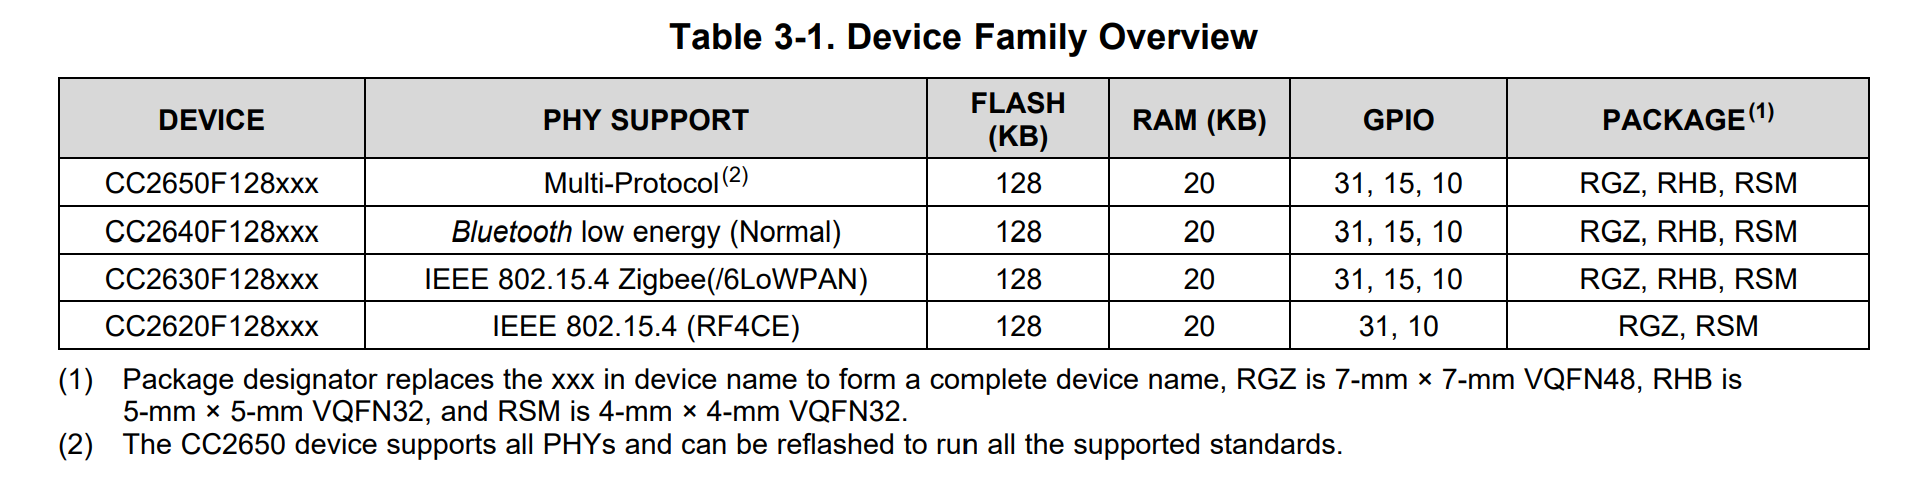
\includegraphics[width=1\textwidth]{media/table26xx.png}
  \caption{TI Device Family}
\end{figure}

Als Koordinator werden die Leistungsfähigeren Chips aus der 265X Reihe eingesetzt. Touchlink ist eine Technologie, um ZigBee Geräte einfach zu koppeln. Dafür setzt
Touchlink Bluetooth LE ein. Die Unterstüzung von diesem Protokoll ist daher vorteilhaft.

\begin{figure}[H]
  \centering
  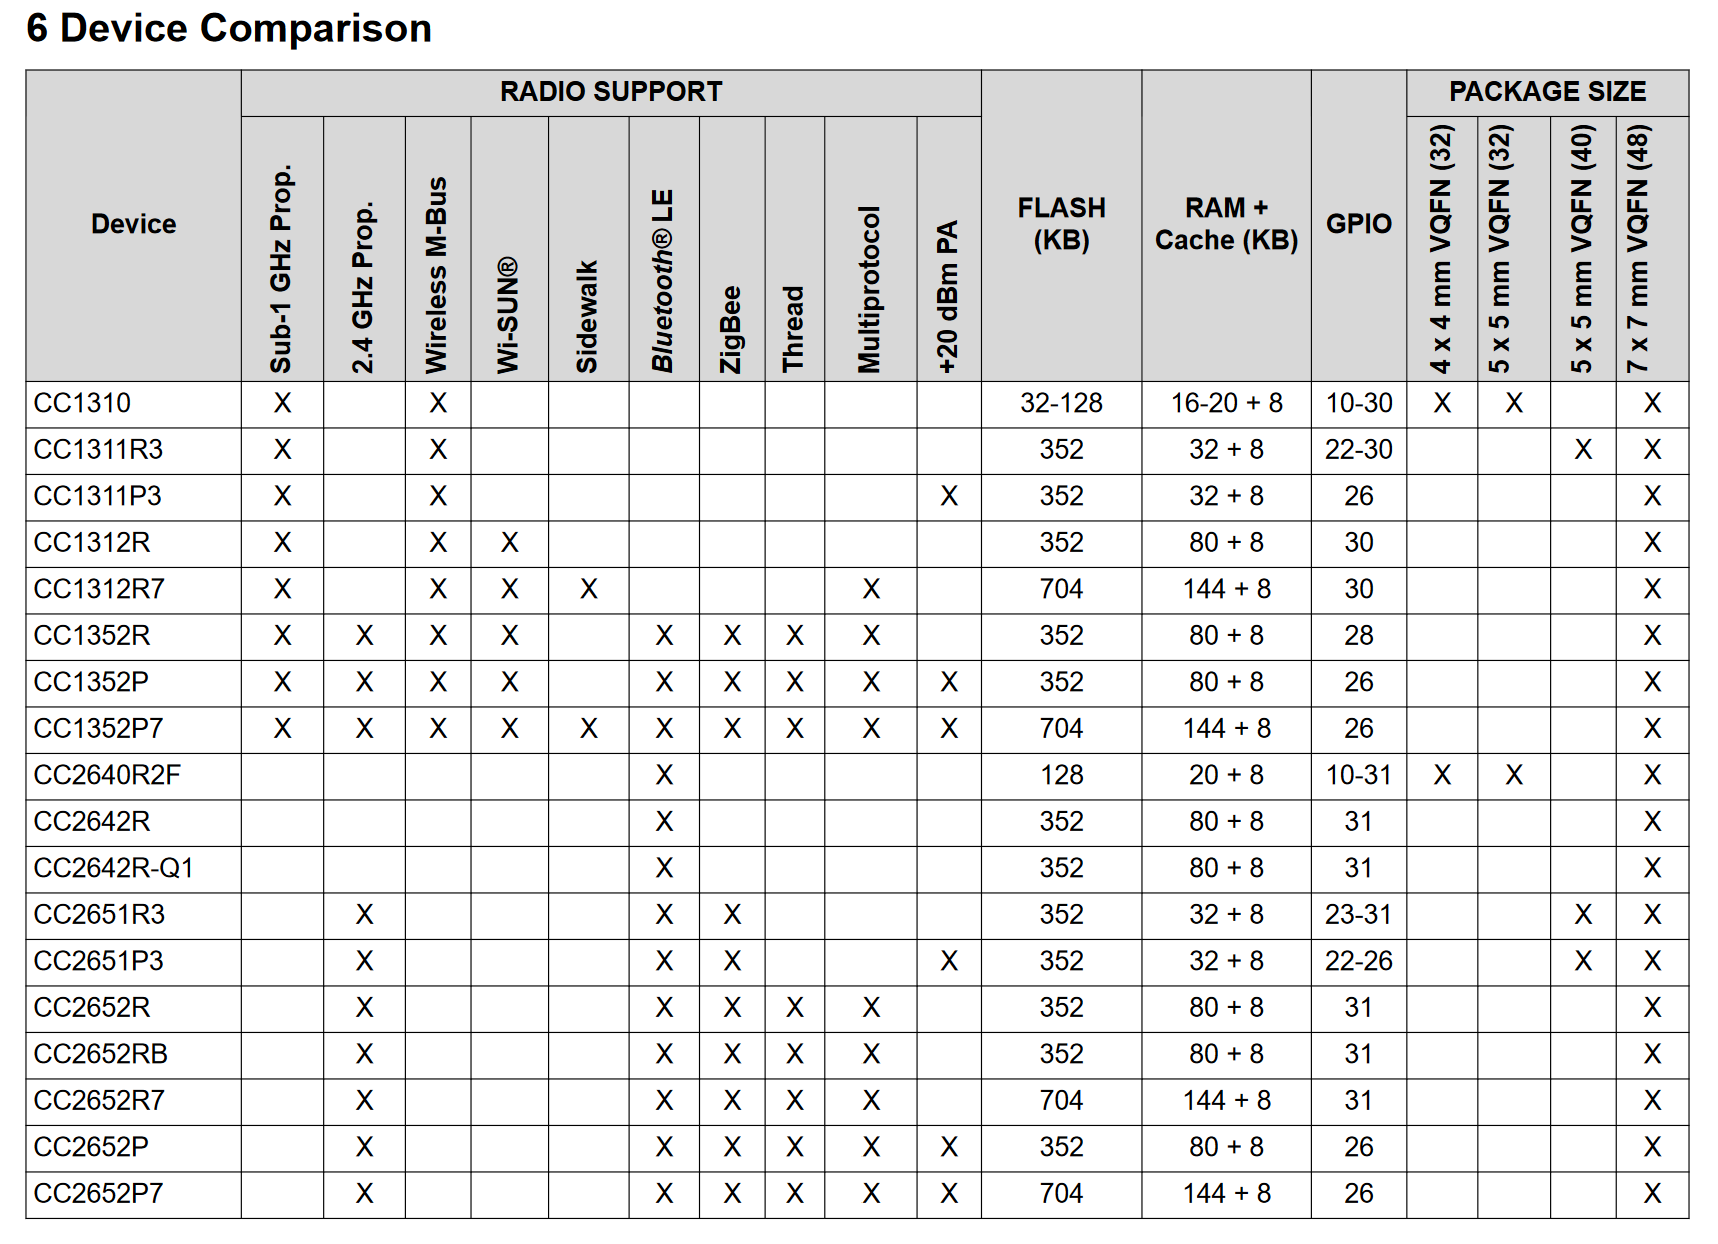
\includegraphics[width=1\textwidth]{media/table265x.png}
  \caption{TI CC 265X Serie}
\end{figure}

In der Tabelle sind die unterstützten Protokolle der einzelnen Modelle sowie deren Leistungsfähigkeit aufgeführt.
Es ist anzumerken, dass die größeren Modelle schon den Standard Thread unterstützen, der vermutlich durch das
Projekt \grqq Matter\grqq{} erheblich an Bedeutung gewinnen wird.

Texas Instruments stellt als Basis für ZigBee Anwendungen eine Bibliothek \grqq Z-Stack\grqq{} zur Verfügung. Diese stellt grundlegenden 
Funktionen um das ZigBee Protokoll zu implementieren zur Verfügung. Mit Texas Instruments Code Composer Studio steht eine IDE bereit,
um den Entwicklungsprozess zu unterstützen. Auf den entsprechend Leistungsfähigeren Chips lassen sich in freie Speicherbereiche noch zusätzliche
Funktionalitäten einprogrammieren. Die Chips können mit Programmierboards des Herstellern programmiert werden. Alternativ kann man
günstig einen USB-Stick mit aufgelöteten CC Chip erwerben, und auch diesem mit entsprechenden Tools programmieren.

Weiter Informationen: \url{https://www.ti.com/tool/Z-STACK#overview}

In dem OpenSource Projekt zigbee2mqtt werden ausschließlich Chips von Texas Instruments unterstützt. Die meißten gängigen Anbieter von Microchips 
haben entsprechende Modelle im Angebot. 

\section{Versuchshardware}

\subsection{RaspberryPi}

Der RaspberryPi ist ein ARM basierter Computer im Mini-Format. Er dient in diesem Versuch als Applikationsserver und gleichzeitig als Versuchs-PC, 
auf dem der Versuch durchgeführt wird. Die eingesetzten Anwendungen sind 
als Webservice implementiert und werden als Container mit Docker betrieben.

Der RaspberryPi besitzt die PC typischen Schnittstellen wie Ethernet, HDMI, und USB. Als Speicher wird eine SD-Karte eingestzt. 

\subsection{RaspberryPi Zigbee Hat}

Als Zigbee Koordinator wird ein auf dem TI CC2652 basierendem RaspberryPi Hat vom Hersteller \grqq cod.m\grqq{} eingesetzt. Dieser wurde vom Hersteller
für den Einsatz mit \grqq homegear\grqq{} oder \grqq zigbee2Mqtt\grqq{} entwickelt. Ein Datenblatt und Bedienungsanleitung sind im Anhang.

\begin{figure}[H]
  \centering
  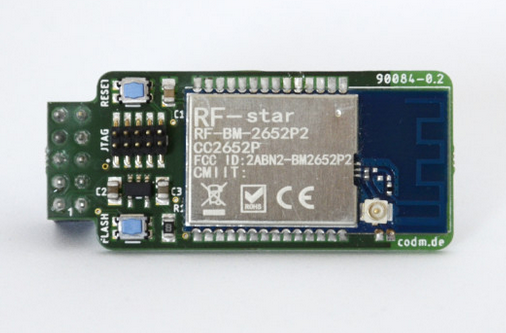
\includegraphics[width=1\textwidth]{media/codm.png}
  \caption{ZigBee cod.m Koordinator \\ Bildquelle: cod.m Produktfoto}
\end{figure}

Durch einen Lötjumper kann zwischen einer aufgedruckten und einer per \grqq ufl\grqq{} angeschlossenen Antenne gewechselt werden.

\subsection{CC2531 Sniffer Stick}

Mit diesem Stick wird die ZigBee Kommunikation des Versuchsnetzwerkes mitgeschnitten.
Der Stick basiert auf einem leistungsschwachen Chip, der mit entsprechender Firmware ZigBee Kommunikation mitschneiden kann. 

Als Treiber wird ein in C geschriebenes Programm verwendet, welches es ermöglicht den Stick direkt als Interface in Wireshark hinzuzufügen. Der Quellcode findet sich in 
GitHub unter https://github.com/andrebdo/wireshark-cc2531. Eine Anleitung zum kompilieren ist im Repository enthalten. Die hieraus entstehende ausführbare Datei muss in ein
entsprechendes Verzeichnis kopiert werden, und kann anschließend als Interface in Wireshark ausgewählt werden. Die Funktion nennt sich bei Wireshark \grqq extcap \grqq{}.

\subsection{Phillips Hue Komponenten}

Unter dem Namen \grqq Hue \grqq{} vertreibt Phillips eine Reihe von vernetzten Endgeräten sowie entsprechende Komponenten um diese zu steuern.
Die Phillips Hue Serie setzt auf ZigBee sowie Bluetooth LE. Unter anderem sind Lampen, Steckdosen, eine Bridge sowie eine App verfügbar.
Die Bridge stellt bei traditionellen Lösungen die Schnittstelle zwischen dem ZigBee Netzwerk und der IP Kommunikation zu einer Smartphone
App oder ähnlichem. Die Endgeräte sind Kompatibel zu dem Software-Gateway zigbee2mqtt, benutzen also keine speziellen Schlüssel.
Die Lampen werden in dem Versuch als Demonstrationsobjekte eingesetzt. Sie können Ein- und Ausgeschaltet werden, sowie gedimmt werden. Zusätzlich wird eine
Phillips Hue Fernbedienung verwendet, die zur Steuerung der Lampen genutzt wird.

\section{Eingesetzte Software}

\subsection{Raspbian OS}

RaspbianOS ist eine leichtgewichtige Linux Distribution, welche direkt vom Hersteller des RaspberryPis speziell auf die Bedürfnisse des Board angepasst ist. Es enthällt eine
Desktop Umgebung sowie grundlegende Pakete. Es basiert auf Debian, damit sind entsprechenden reichhaltige Paketquellen verfügbar. 

\subsection{Docker}

Docker ist eine Containerisierungslösung, um Anwendungen containerisiert auf Linux-Servern ausführen zu können. Docker reduziert erheblich den Aufwand 
Anwendungen zu betreiben. Docker Container beinhalten alle Abhängigkeiten um die Anwendung im Container lauffähig zu machen.
Prozesse laufen in eigenen Namespaces und sind dadurch abgekoppelt von anderen Containern sowie dem Hostbetriebssystem. Im Unterschied zur Virtualisierung werden
einige Ressourcen gemeinsam genutzt. Dadurch ist die Effizienz höher als bei taditioneller Virtualisierung, bei der ein vollständiges Betriebssystem virtualisiert wird.

\subsection{Docker-Compose}

Docker-Compose ist ein Tool, um Containerumgebungen im Textformat, hier \grqq YAML \grqq{}, zu beschreiben.
Ein Container kann im einfachen Fall per Docker-CLI mit entsprechenden Parametern gestartet werden:
\begin{lstlisting}
  docker run hello-world -v ./home:/home -p 80:80
\end{lstlisting}

Durch diesen Befehl wird der Container \grqq hello-world \grqq aus dem Docker Repository geladen und anschließend gestartet. In diesem ist ein einfacher Webserver der bei
Aufruf ein \grqq Hello world ! \grqq{} zurückgibt implementiert. Zusätzlich wird der Ordner \grqq home \grqq{} in den Container gemountet. Dieser bleibt auch bei einem
erneuten Laden des Containers persistent. Dies wird beispielweiße für Konfigurationsdateien oder andere persistente Dateien genutzt. Um den Container auch auf der Schnittstelle
des Host-Systems verfügbar zu machen, wird der Port 80 auf den Container Port 80 gemappt. Die Funktionsweise wird später erläutert.

Als handliche Alternativ zu der Docker-CLI lässt sich der Zielzustand auch in einer Textdatei beschreiben:

\begin{lstlisting}
version: '3'
services:
  helloworld:
    container_name: helloworld
    image: hello-world
    ports:
      - 80:80
    volumes:
      - ./home:/home
    restart: unless-stopped
\end{lstlisting}

Mit einem 
\begin{lstlisting}
  docker-compose up -d
\end{lstlisting}

errhält man das selbe Ergebniss wie mit dem vorher gezeigtem CLI Befehl.

\subsection{zigbee2mqtt}

\begin{figure}[H]
  \centering
  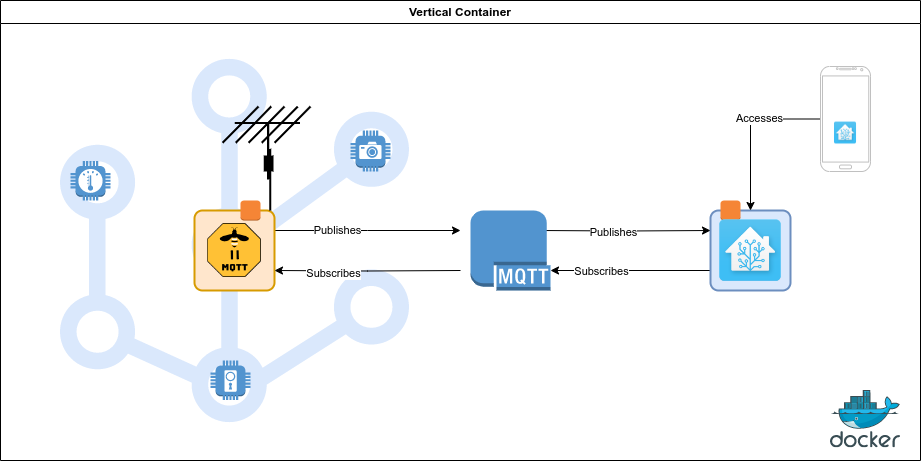
\includegraphics[width=1\textwidth]{media/z2m-arch.png}
  \caption{Zigbee2Mqtt Kontext}
\end{figure}

zigbee2mqtt ist ein offenes Softwareprojekt und kann am besten mit dem Begriff \grqq Software-Zigbee-Gateway\grqq{} beschrieben werden. Es übernimmt die Funktionalität, die normalerweise entsprechende
Bridges der Hersteller übernehmen. Während traditionelle Bridges, wie zum Beispiel die Phillips Hue Bridge eine REST API zur Verfügung stellen um mit entsprechenden
Apps zu kommunizieren, macht zigbee2mqtt die Geräte per mqtt nach außen verfügbar. Auf abstrakter Ebene bedeutet dies, dass es ein Gateway zwischen einem Zigbee Netzwerk und
einem traditionellen IPv4 Netzwerk ist. Zur Steuerung und Visualisierung lassen sich per MQTT Anwendungen wie \grqq Homeassistant\grqq{} oder \grqq OpenHUB\grqq{} oder auch entsprechende
Eigenentwicklungen einsetzen. \grqq zigbee2mqtt\grqq{} greift direkt auf den \grqq cod.m\grqq{} ZigBee Adapter zu.

Quellcode und Dokumentation: \url{https://github.com/Koenkk/zigbee2mqtt}
Homepage: \url{https://www.zigbee2mqtt.io/}

\grqq zigbee2mqtt\grqq{} verwaltet ein Zigbee Netzwerk und ermöglicht es Drittanwendungen, die Geräte in diesem ZigBee Netz zu Steuern. Wird ein neues Device ins das Netzwerk eingefügt, 
kündigt zigbee2mqtt das Gerät per MQTT an, und teilt der Anwendunge nach erfolgreichem Interview die verfügbaren Cluster des neuen Teilnehmers mit.

Zigbee2Mqtt verwaltet drei Datenbanken, welche die Funktionsweiße deutlich machen. Viele Funktionen, wie zum Beispiel die Verwaltung von Routingtabellen und
Verschlüsselung der Kommunikation sind direkt in der Hardware implementiert. Diese Funktionen lassen sich wie in der im Punkt TI CC Firmware gezeigen API Steuern und Abfragen.
Zigbee2mqtt verwaltet in einer eigenen Datenbank die Geräte im Netzwerk sowie deren Eigenschaften.
Folgende Datensätze finden sich in der Anwendung:

\textbf{coordinator-backup.json}\\

Hier sind die für die Initialisierung beim Start des Koordinators wichtigen Informationen abgelegt. Dies beinhaltet alle dem Netzwerk zugehörigen Geräte.
Durch löschen dieser Datei wird das Netzwerk vollständig zurückgesetzt. Die einzelnen Teilnehmer müssen dann manuell per Touchlink oder nach herstellerspezifischem Verfahrem
zurückgesetzt werden, um wieder einem neuen Netzwerk beitreten zu können.


\begin{lstlisting}
  {
    "metadata": {
      "format": "zigpy/open-coordinator-backup",
      "version": 1,
      "source": "zigbee-herdsman@0.14.103",
      "internal": {
        "date": "2023-05-04T19:48:28.936Z",
        "znpVersion": 1
      }
    },
    "stack_specific": {
      "zstack": {
        "tclk_seed": "69a6670050d8354347405537724e1a81"
      }
    },
    "coordinator_ieee": "00124b0026b748c8",
    "pan_id": "1a62",
    "extended_pan_id": "00124b0026b748c8",
    "nwk_update_id": 0,
    "security_level": 5,
    "channel": 11,
    "channel_mask": [
      11
    ],
    "network_key": {
      "key": "01030507090b0d0f00020406080a0c0d",
      "sequence_number": 0,
      "frame_counter": 5552161
    },
    "devices": [
      {
        "nwk_address": "9a3b",
        "ieee_address": "0017880104b9359d",
        "is_child": false,
        "link_key": {
          "key": "87b4d0a2668847d8a876fe4454bf654e",
          "rx_counter": 0,
          "tx_counter": 121
        }
      },
  ...  
  \end{lstlisting}

  \textbf{state.json}\\

  In dieser Datei sind alle aktuellen Zustände Geräte im Netzwerk hinterlegt. Sie dient dazu, bei einem Neustart des Koordinators den letzten Zustand wieder herzustellen.

  \begin{lstlisting}
    ...
    "0xbc33acfffe9587ed": {
        "brightness": 15,
        "state": "OFF",
        "color_mode": "color_temp",
        "color_temp": 360,
        "linkquality": 40,
        "color": {
            "x": 0.4542,
            "y": 0.4092
        },
        "do_not_disturb": false
    ...
  \end{lstlisting}
  \textbf{database.db}\\

  Dies ist die zentrale Datenbank von zigbee2mqtt. Da SQLite eingesetzt wird, lässt sich auch hier der Inhalt wie bei einer Textdatei einfach auslesen.
  Es liegt für jedes Device ein Datensatz ab.

  Datensatz des Koordinators:
  \begin{lstlisting}
{"id":1,"type":"Coordinator","ieeeAddr":"0x00124b0026b748c8","nwkAddr":0,"manufId":0,"epList":[1,2,3,4,5,6,8,10,11,12,13,47,110,242],
"endpoints":{"1":{"profId":260,"epId":1,"devId":5,"inClusterList":[],"outClusterList":[],"clusters":{},"binds":[],"configuredReportings":[],
"meta":{}},"2":{"profId":257,"epId":2,"devId":5,"inClusterList":[],"outClusterList":[],"clusters":{},"binds":[],"configuredReportings":[],
"meta":{}},"3":{"profId":260,"epId":3,"devId":5,"inClusterList":[],"outClusterList":[],"clusters":{},"binds":[],"configuredReportings":[],
"meta":{}},"4":{"profId":263,"epId":4,"devId":5,"inClusterList":[],"outClusterList":[],"clusters":{},"binds":[],"configuredReportings":[],
"meta":{}},"5":{"profId":264,"epId":5,"devId":5,"inClusterList":[],"outClusterList":[],"clusters":{},"binds":[],"configuredReportings":[],
"meta":{}},"6":{"profId":265,"epId":6,"devId":5,"inClusterList":[],"outClusterList":[],"clusters":{},"binds":[],"configuredReportings":[],
"meta":{}},"8":{"profId":260,"epId":8,"devId":5,"inClusterList":[],"outClusterList":[],"clusters":{},"binds":[],"configuredReportings":[],
"meta":{}},"10":{"profId":260,"epId":10,"devId":5,"inClusterList":[],"outClusterList":[],"clusters":{},"binds":[],"configuredReportings":[],
"meta":{}},"11":{"profId":260,"epId":11,"devId":1024,"inClusterList":[1281,10],"outClusterList":[1280,1282],"clusters":{},"binds":[],"configuredReportings":[],
"meta":{}},"12":{"profId":49246,"epId":12,"devId":5,"inClusterList":[],"outClusterList":[],"clusters":{},"binds":[],"configuredReportings":[],
"meta":{}},"13":{"profId":260,"epId":13,"devId":5,"inClusterList":[25],"outClusterList":[],"clusters":{},"binds":[],"configuredReportings":[],
"meta":{}},"47":{"profId":260,"epId":47,"devId":5,"inClusterList":[],"outClusterList":[],"clusters":{},"binds":[],"configuredReportings":[],
"meta":{}},"110":{"profId":260,"epId":110,"devId":5,"inClusterList":[],"outClusterList":[],"clusters":{},"binds":[],"configuredReportings":[],
"meta":{}},"242":{"profId":41440,"epId":242,"devId":5,"inClusterList":[],"outClusterList":[],"clusters":{},"binds":[],"configuredReportings":[],
"meta":{}}},"interviewCompleted":true,"meta":{},"lastSeen":1671278654240,"defaultSendRequestWhen":"immediate"}

  \end{lstlisting}

In dieser Datenbank sind alle Geräte, welche direkt mit dem Koordinator verbunden sind vermerkt. Zu jedem Gerät werden die gebundenen Cluster vermerkt.

\subsubsection{zigbee-herdsman}

Der Herdsman ist die eigentliche Kernanwendung von zigbee2mqtt. Diese Modul verbindert sich direkt über einen seriellen Socket mit dem Koordinator. Über diese Schnittstelle
spricht Herdsmann die API des Koordinators an um das Netzwerk zu verwalten. Herdsman verwaltet die Datenbank und damit den Zustand des Netzwerkes. Das Modul stellt nach außen
eine API zur Verfügung, mit der Sich das Netzwerk verwalten lassen kann. Auf diese API greift auch die integrierte WebGui zu.

Die API von zigbee-herdsman wird im entsprechenden GitHub Repository dokumentiert.
\url{https://github.com/Koenkk/zigbee-herdsman}

\subsubsection{zigbee-herdman-converters}

Dieser Konverter kann proprietäre Cluster die von selbstentwickelten Devices oder manch Devices von Drittherstellern. Mit diesem Converter lassen sich proprietäre Cluster von Geräte
so adaptieren, dass sie nach Wunsch gesteuert und ausgelesen werden können.

\subsubsection{zigbee2mqtt}

Dieses Modul umschreibt die beiden vorher beschriebenen Module und umfasst noch eine Weboberfläche. Die Weboberfläche dient zur Verwaltung und Visualisierung des Netzwerkes.
\begin{figure}[H]
  \centering
  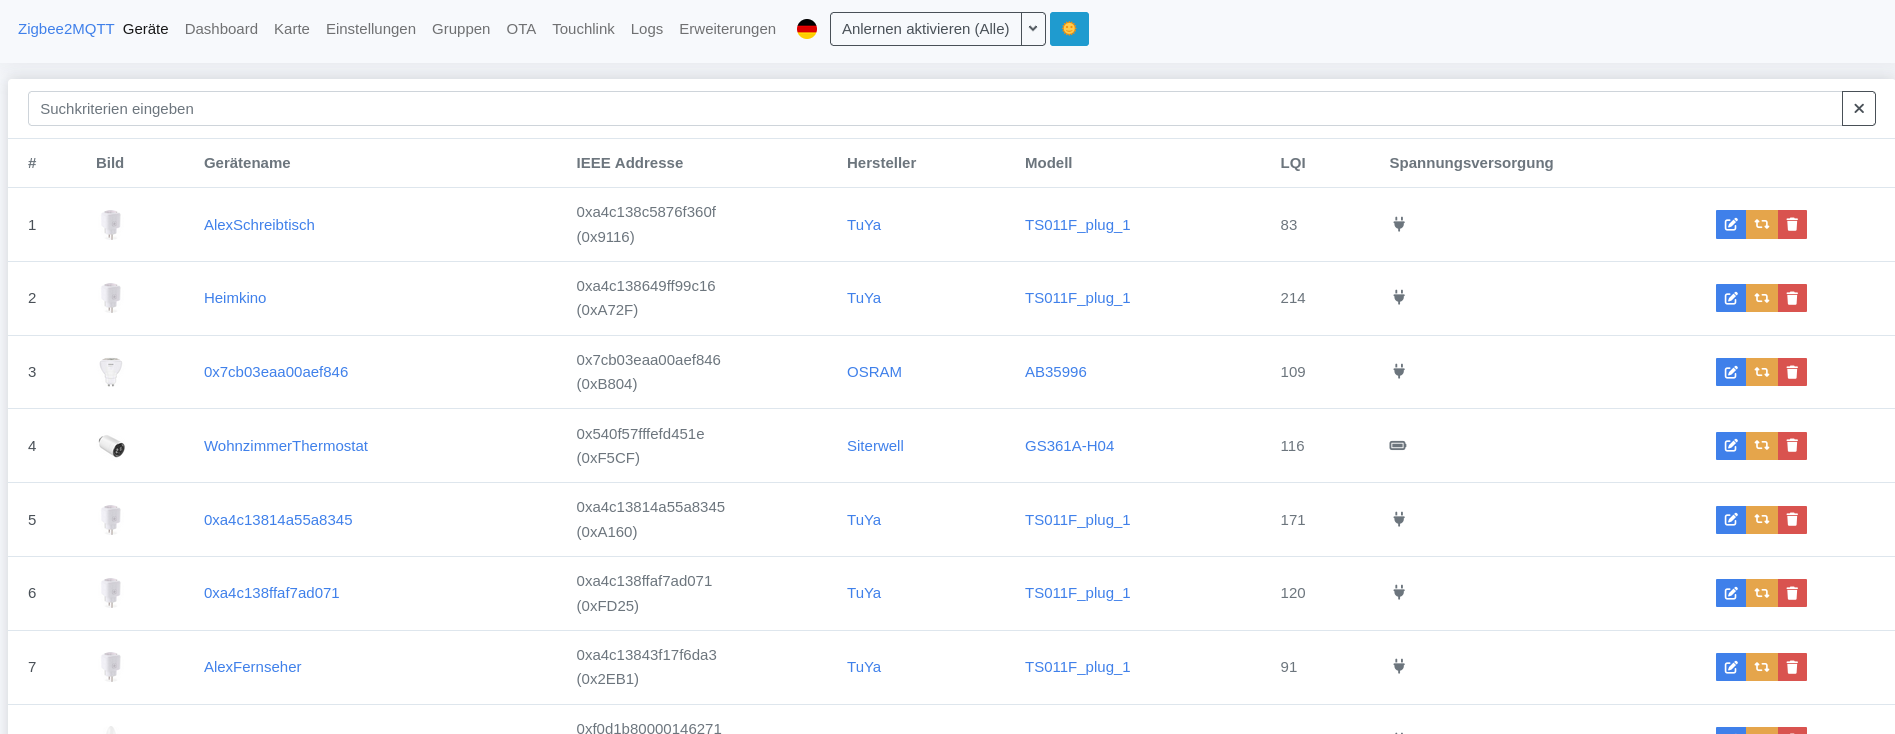
\includegraphics[width=1\textwidth]{media/z2m.png}
  \caption{zigbee2mqtt Webfrontend}
\end{figure}

Die Weboberfläche biete die Möglichkeit alle Endpunkte von Herdsman abzufragen und entsprechend zu steuern.

\begin{figure}[H]
  \centering
  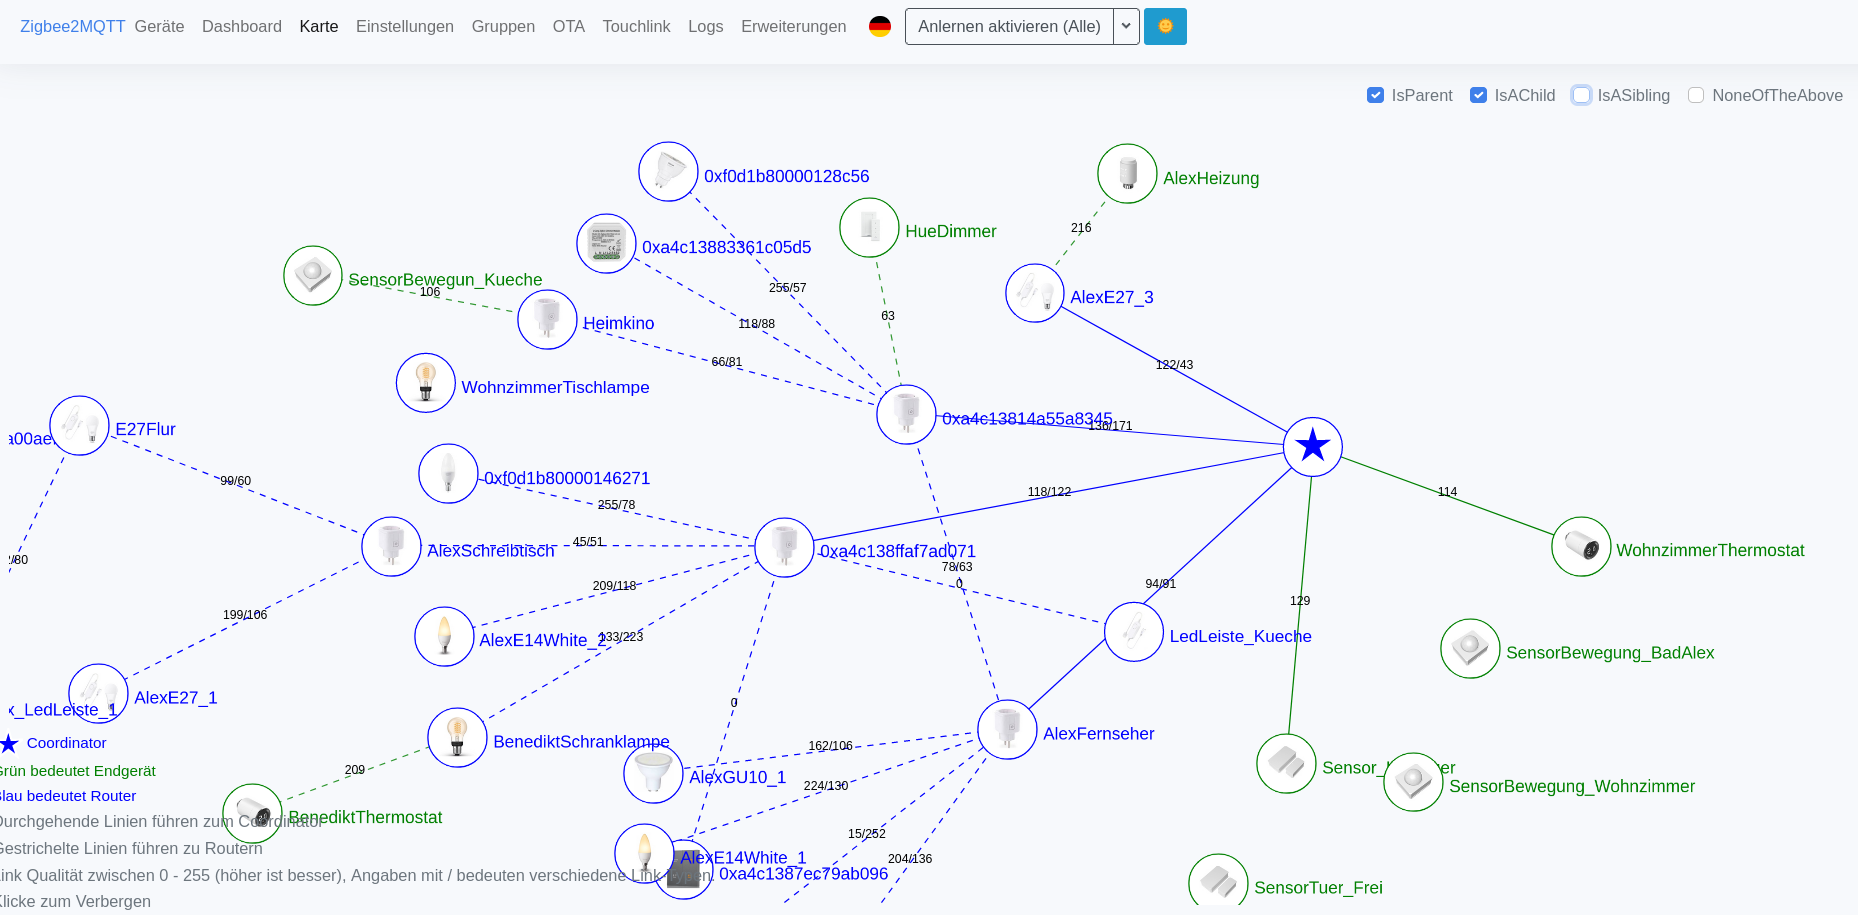
\includegraphics[width=1\textwidth]{media/z2m-map.png}
  \caption{zigbee2mqtt Netzwerkvisualisierung}
\end{figure}

Das Netzwerk lässt sich in einer dynamischen Übersicht visualisieren. Hier die aktiv genutzen Verbindung zwischen den Geräten. 


\subsubsection{TI CC Firmware}

Eine Firmware für die Texas Instruments Chips, um diese als Koordinator einsetzen zu können. Die Firmware basiert auf dem Z-Stack von Texas Instruments. Sie wird fertig kompiliert
in dem Git-Repo von zigbee2mqtt angeboten. Sie kann auf die USB-Koordinatoren per USB geflasht werden, der Einsatz eines Launchpads ist nicht notwendig. Eine Anleitung
findet sich auf der Homepage von zigbee2mqtt.  


Zur Veranschaulichung der Funktionsweiße, ein Ausschnitt aus der API Dokumentation:

\begin{figure}[H]
  \centering
  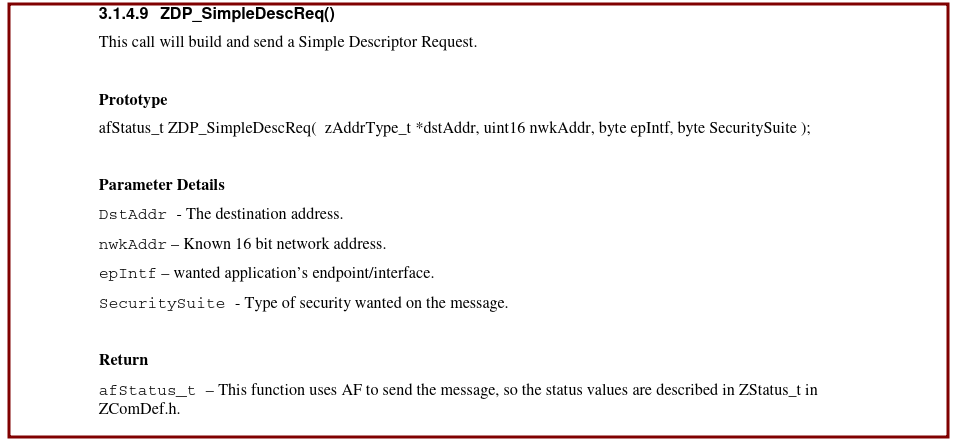
\includegraphics[width=1\textwidth]{media/z-stack-api-excerpt.png}
  \caption{Z-Stack API Auszug}
\end{figure}

In diesem Beispiel wird beschrieben, wie man einen SimpleDescriptor-Request an ein Zigbee-Device versendet. Dieser Aufruf ist entsprechend parametrierbar,
und wird zur Abfrage der verfügbaren Endpunkte eines Gerätes nach dessen Beitritt in das Netzwerk abgefragt.

Die Firmware, die auf dem Koordinator zum Einsatz kommt basiert auf einem Beispiel Projekt für einen ZigBee Koordinator von Texas Instruments. Dieses ist
im SDK Kit des TI CC2652 Chips enthalten, und kann mit dem Texas Instruments Code Compose Studio bearbeitet werden. Die Firmware kann selbst kompiliert werden.
Dazu kann ein Git Patch von den Maintainern von zigbee2mqtt angewendet werden. Zusätzlich können nun eigene Änderungen in den Code einfließen. Der Patch ist unter
folgender URL zu finden.
\url{https://github.com/Koenkk/Z-Stack-firmware/blob/master/coordinator/Z-Stack_3.x.0/firmware.patch} .
Die Änderungen, die vorgenommen werden können hier nachgelesen werden. Eine Anleitung zum kompilieren liegt ebenfalls im Git Repository ab.

\begin{figure}[H]
  \centering
  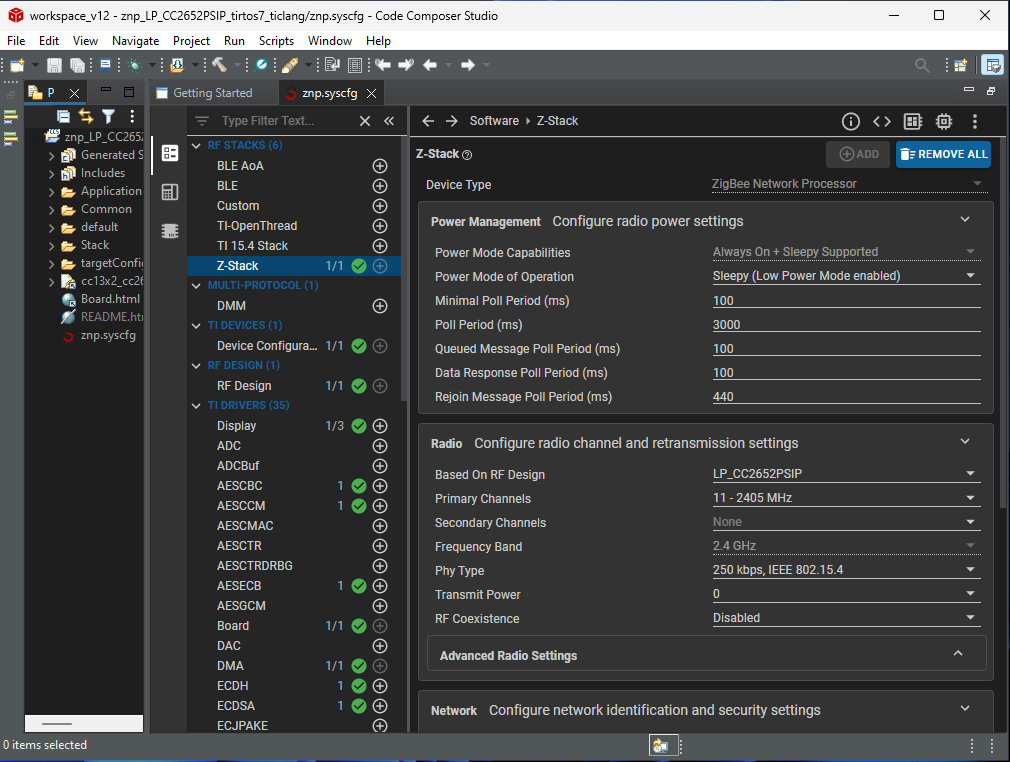
\includegraphics[width=1\textwidth]{media/cc-device.png}
  \caption{TI Code Compose Studio}
\end{figure}
In der Abbildund ist das geöffnete Projekt im Code Compose Studio mit den verschiedenen Konfigurationen die vorgenommen werden können.

\subsection{MQTT}

MQTT \cite{mqtt} ist ein Protokoll, um Nachrichten zwischen Teilnehmen in einem IP Netzwerk auszutauschen. Alle Nachrichten werden unter einem definierten \grqq Topic \grqq{} 
an einen zentralen Messagebroker gesendet. Teilnehmer können \grqq Topics \grqq{} abonnieren. Der Broker verwaltet eine Liste mit allen Teilnehmern sowie 
deren abonnierten \grqq Topics \grqq{}. Wird eine entsprechende Nachricht an den Broker gesendet, werden alle Abonennten des Topics entsprechend informiert.
In dem Versuch wird der quelloffene MQTT Broker \grqq mosquitto\grqq{} eingesetzt. 

\subsection{Wireshark}

Wireshark ist eine quelloffene Anwendung um Datenstöme mitzuschneiden und zu untersuchen. Wireshark selbst nutzt standardmäßig \grqq npcap \grqq{} um Datenverkehr 
auf Netzwerkkarten aufzuzeichnen. Es ist möglich über andere Schnittstellen Wireshark Datenströme zur Verfügung zu stellen. Zu diesem Zweck
können ausführbare Dateien in einen Ordner \grqq .../extcap \grqq{} abgelegt werden, welche 
Paketströme zurückliefern. 

\begin{figure}[H]
  \centering
  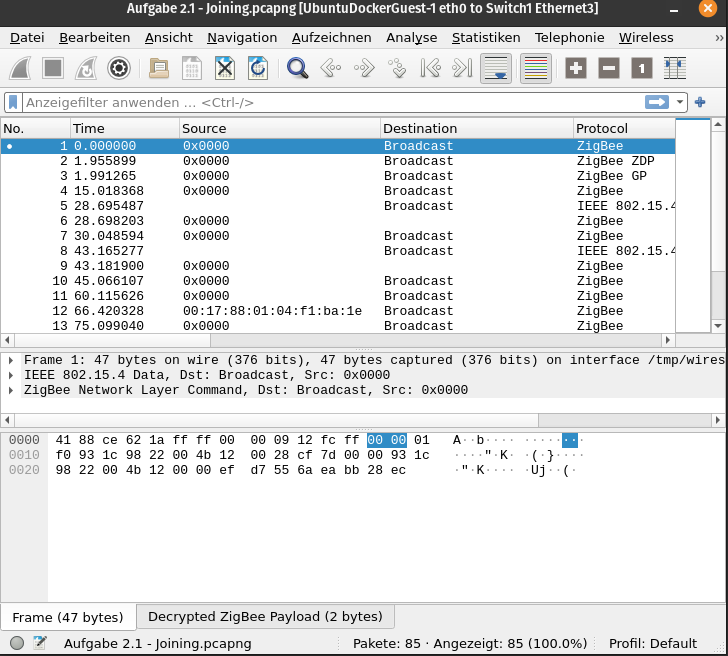
\includegraphics[width=1\textwidth]{media/wireshark.png}
  \caption{Wireshark}
\end{figure}

\subsection{Ansible}

Ansible ist ein Werkzeug zur Automatisierung. Arbeitsabläufe lassen sich strukturiert in YAML (yet another markup language) definieren. Dies ist eine alternative zum schreiben
von Shell Scripten. Ansible kann Aufgaben auf dem lokalem System und auf Remotesystemen ausführen. Aufgaben können in Rollen zusammengefasst werden.  
Eine Rolle kann einem Host wie folgt zugewiesen werden:
\begin{lstlisting}
  - name: Deploy the Lab
    hosts: localhost
    roles:
    - DeployDocker
    - DeployLabUtils
\end{lstlisting}

Die Rollen \grqq DeployDocker \grqq{} und \grqq DeployLabUtils \grqq{} umfassen eine Menge von Aufgaben zur Installation notwendiger Komponenten und weitere Vorbereitungen
für den Praktikumsversuch. Diese Rollen werden \grqq localhost \grqq{}, also dem ausführendem System selbst zugewiesen.
Aus technischer Sicht lädt Ansible parametrierte Pythonmodule auf den jewiligen Host per SCP und führt diese dort aus.



\include{chapter/versuchsdurchführung}
\chapter{Life Cycle Management}
\section{Deployment}
In diesem Kapitel geht es um die Pflege, die Bereitstellung sowie das Zurücksetzen des Praktikumversuchs. Sämtliche Schritte wurden mit Ansible-Playbooks
automatisiert.

Folgende Schritte müssen ausgeführt werden, um ein RaspberryPi vorzubereiten.
\begin{itemize}
    \item Installation von Raspbian OS
    \item Anlegen eines Users
    \item Klonen des GitHub Repositorys nlab4hsrm zigbeelab
\end{itemize}

Zum Ausrollen werden die Rollen \grqq Docker\grqq{} und \grqq ZigbeeLab\grqq{} zugewießen. Dies geschieht durch die DeployLabl.yaml.
\begin{lstlisting}
    ansible-playbook DeployLab.yaml -K -e "channel=<channelnumber>"
\end{lstlisting}

Anschließend wird
\begin{itemize}
    \item Docker Installiert.
    \item Die /etc/hosts Einträge gesetzt.
    \item Die Docker Umgebung vorbereitet.
    \item Die Versuchsumgebung mit allen Komponenten gestartet.
\end{itemize}

\section{Zurücksetzen des Versuchs}

Zum zurücksetzen wird das Playbook \grqq ResetLab\grqq{} ausgeführt.

\begin{lstlisting}
    ansible-playbook ResetLab.yaml -K -e "channel=<channelnumber>"
\end{lstlisting}

\section{Update der eingesetzten Software}

Die RaspberryOS Pakete können mit dem Paktetmanager apt aktuell gehalten werden. Docker zieht initial die Container aus Dockerhub.
Mit folgendem Befehl überprüft Docker das Repository auf aktuelle Container.

\begin{lstlisting}
    docker compose pull /srv/docker-compose.yaml
\end{lstlisting}

Anschließend können die Container mit folgendem Befehl neu gestartet werden.

\begin{lstlisting}
    docker compose up -d /srv/docker-compose.yaml
\end{lstlisting}

\section{Troubleshooting}

Es empfiehlt sich bei Problemen sich den Log der Container anzuschauen.

\begin{lstlisting}
    docker attach <container-name>
\end{lstlisting}

In der Regel ist es am sinnvollsten, mit dem Log von zigbee2mqtt zu starten. Dieser ist erfahrungsgemäßg bei einer Fehlersuche sehr hilfreich.









% Neue leere Seite erzeugen
\newpage
\thispagestyle{empty}
\quad %\addtocounter{page}{-1}
\newpage






%----------------- ANHANG (ROMAN) -------------%
\pagestyle{plain}
\pagenumbering{Roman}

%----------------- VERZEICHNISSE II ---------------------- %


% ----- Abbildungen ----- %
%\addcontentsline{toc}{section}{Abbildungsverzeichnis} % falls in Inhalsverzeichnis
\listoffigures
\clearpage

%----------------- Literaturverzeichnnis ------------------%
\printbibliography
\addcontentsline{toc}{chapter}{Literatur}


\end{document}